\chapter{Android}
In this chapter we will talk about the two applications used by the different users to communicate with the server.

\section{Settings}
First, for this two applications we designed a preference activity which allows the user to change different values to access the server. Indeed the address, the port and the servlet to use can be changed.

\begin{figure}[h!]
  	\centering
    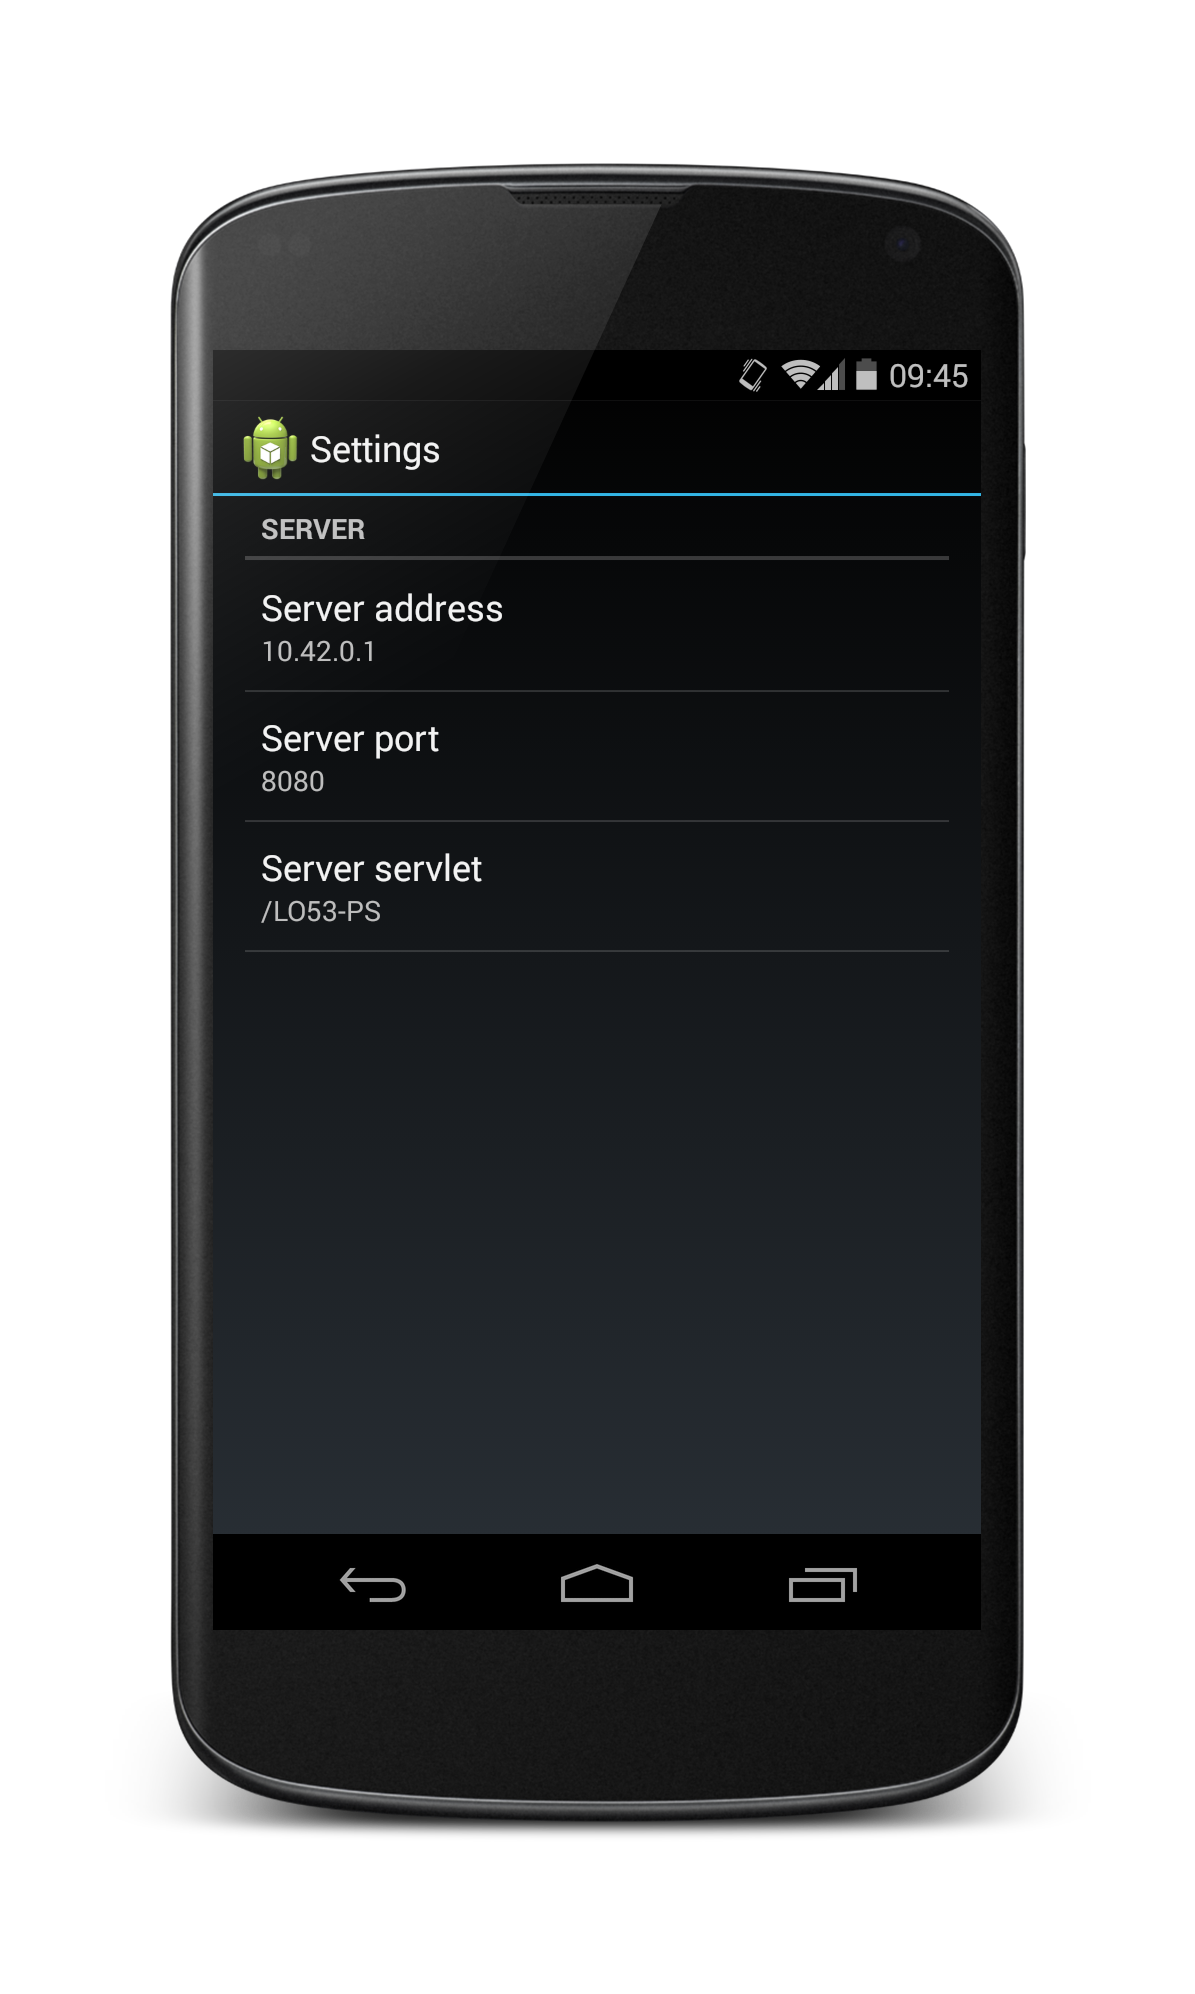
\includegraphics[scale=0.1]{./android/Settings.png}
  \caption{Settings activity}
\end{figure}


\section{Setup Tool}
Now, we will talk about the setup tool application which allows a network administrator for example to set some calibration points in the building. On the next figure you can see the different phase to use this application.


\begin{figure}[h]
        \centering
        \begin{subfigure}[b]{0.3\textwidth}
    			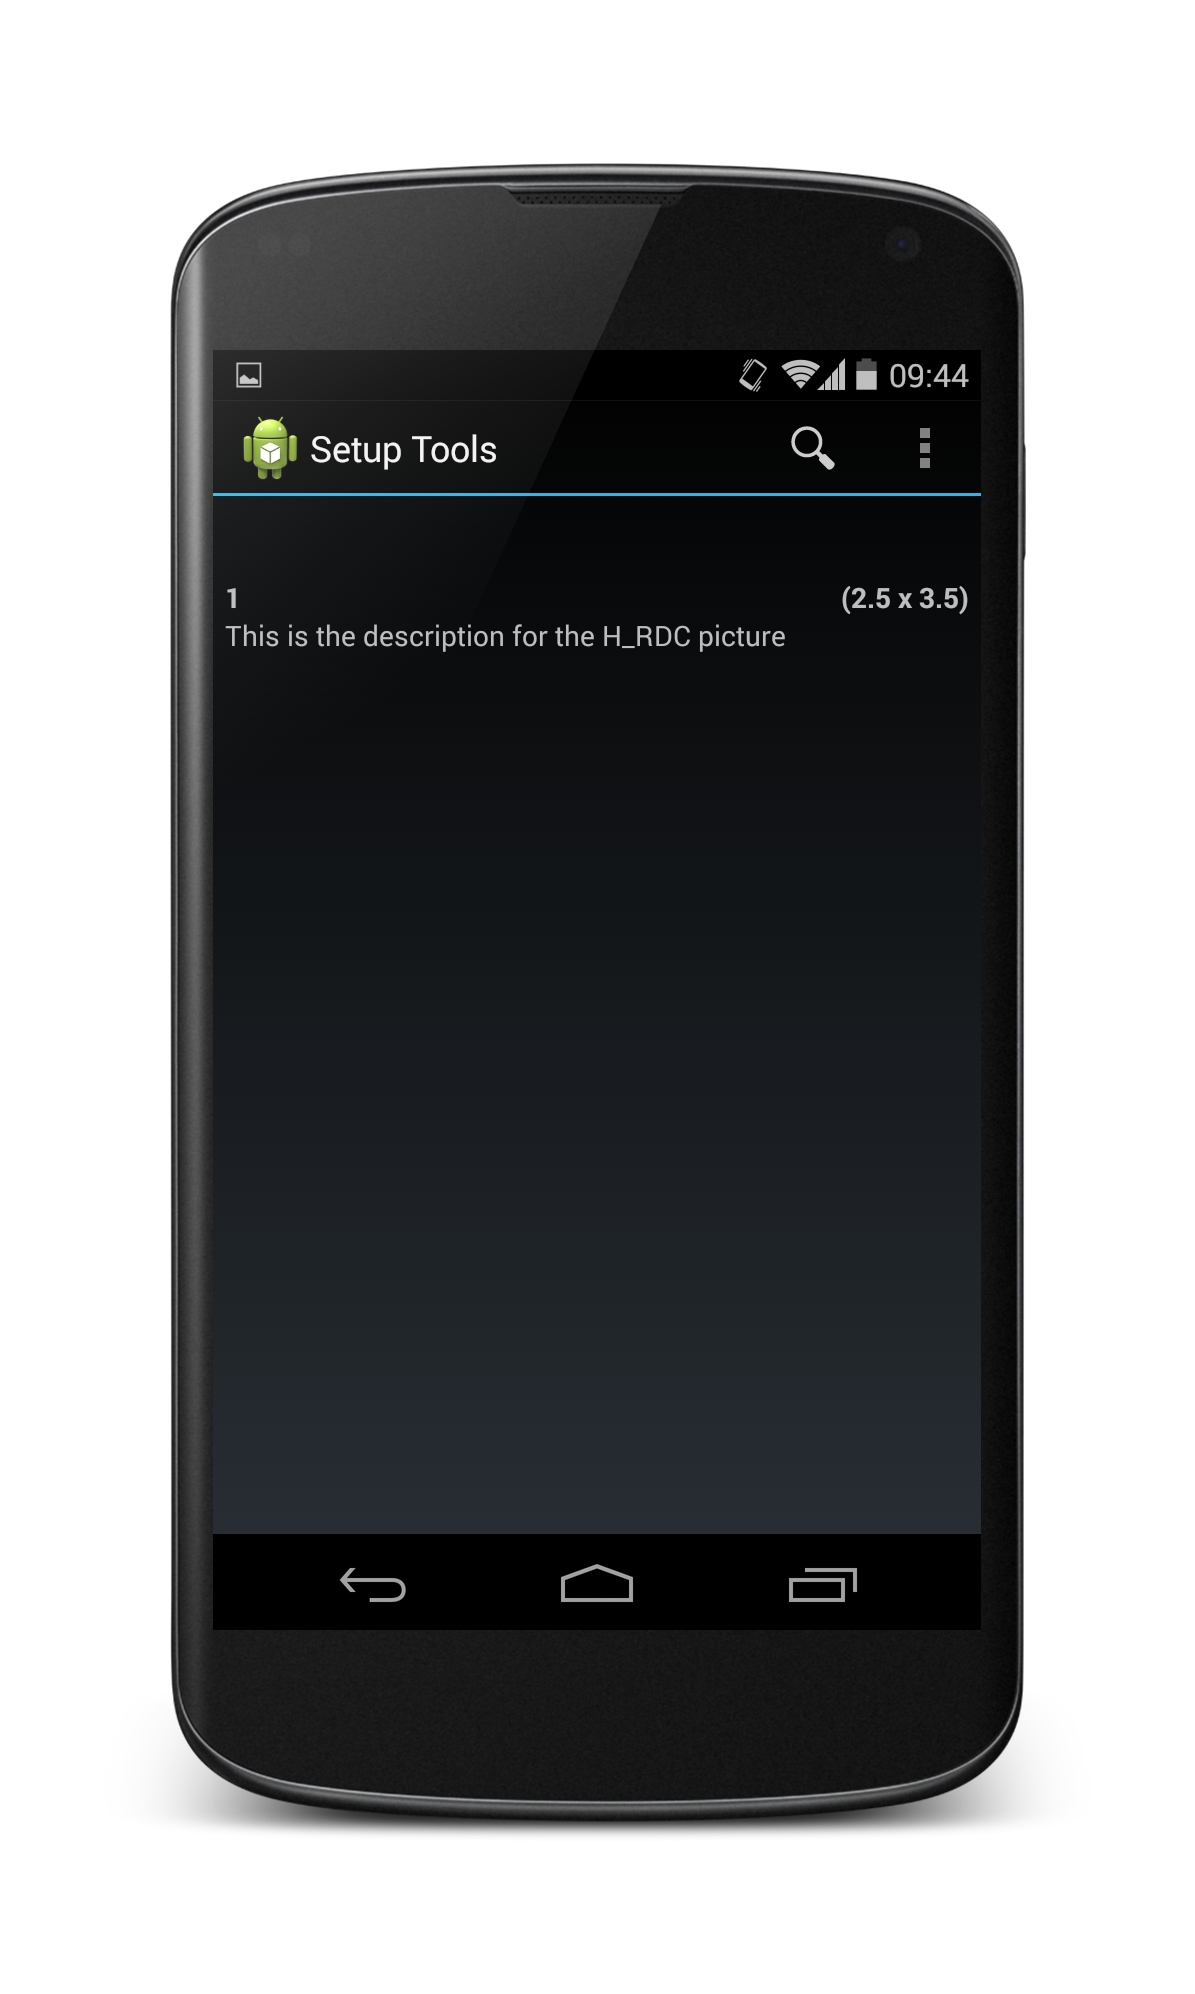
\includegraphics[scale=0.1]{./android/Setup_list.png}
                \caption{Choose your map}
                \label{fig:map_list}
        \end{subfigure}
        \begin{subfigure}[b]{0.3\textwidth}
                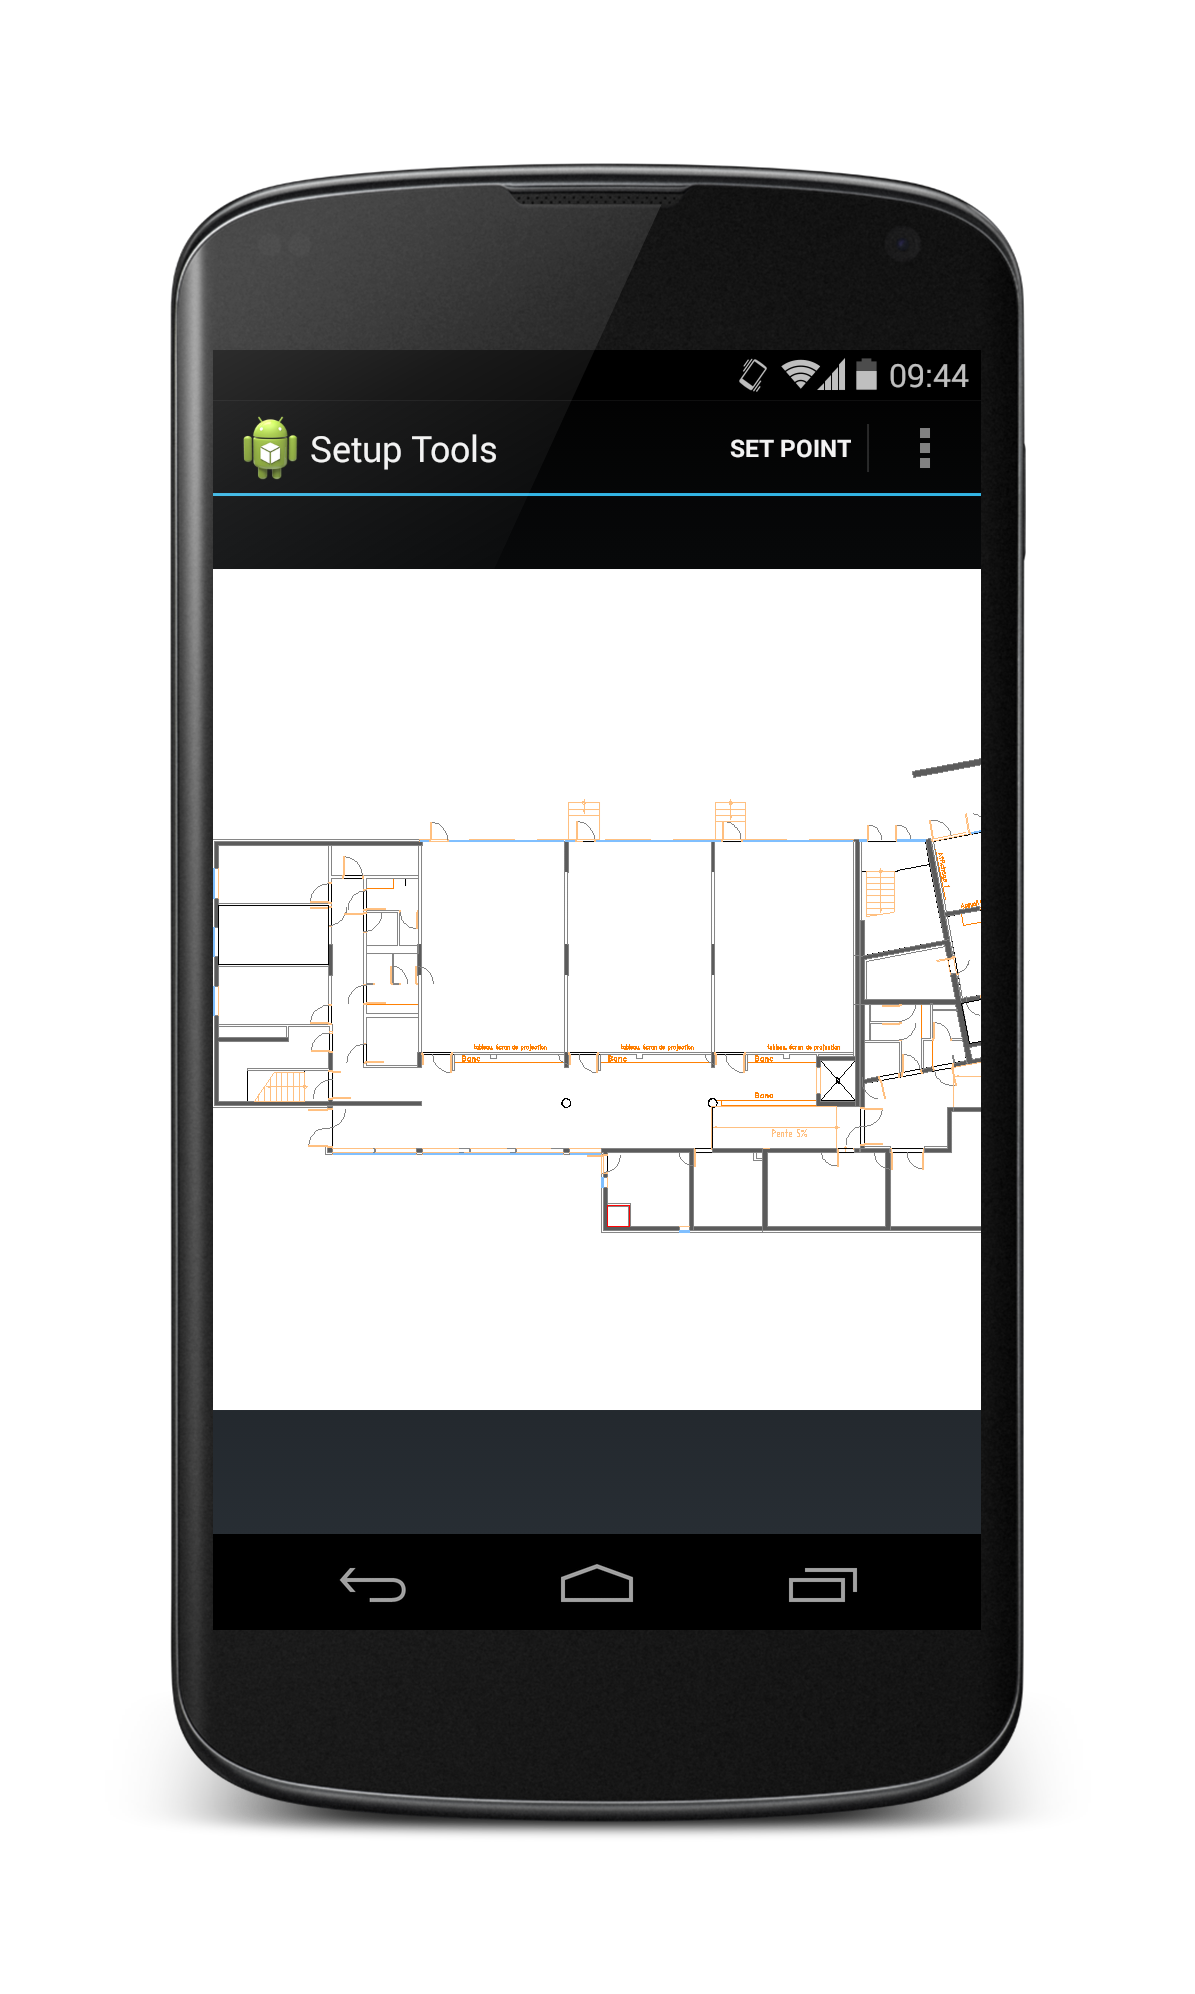
\includegraphics[scale=0.1]{./android/Setup_set.png}
                \caption{Display the map}
                \label{fig:map_set}
        \end{subfigure}
        \begin{subfigure}[b]{0.3\textwidth}
                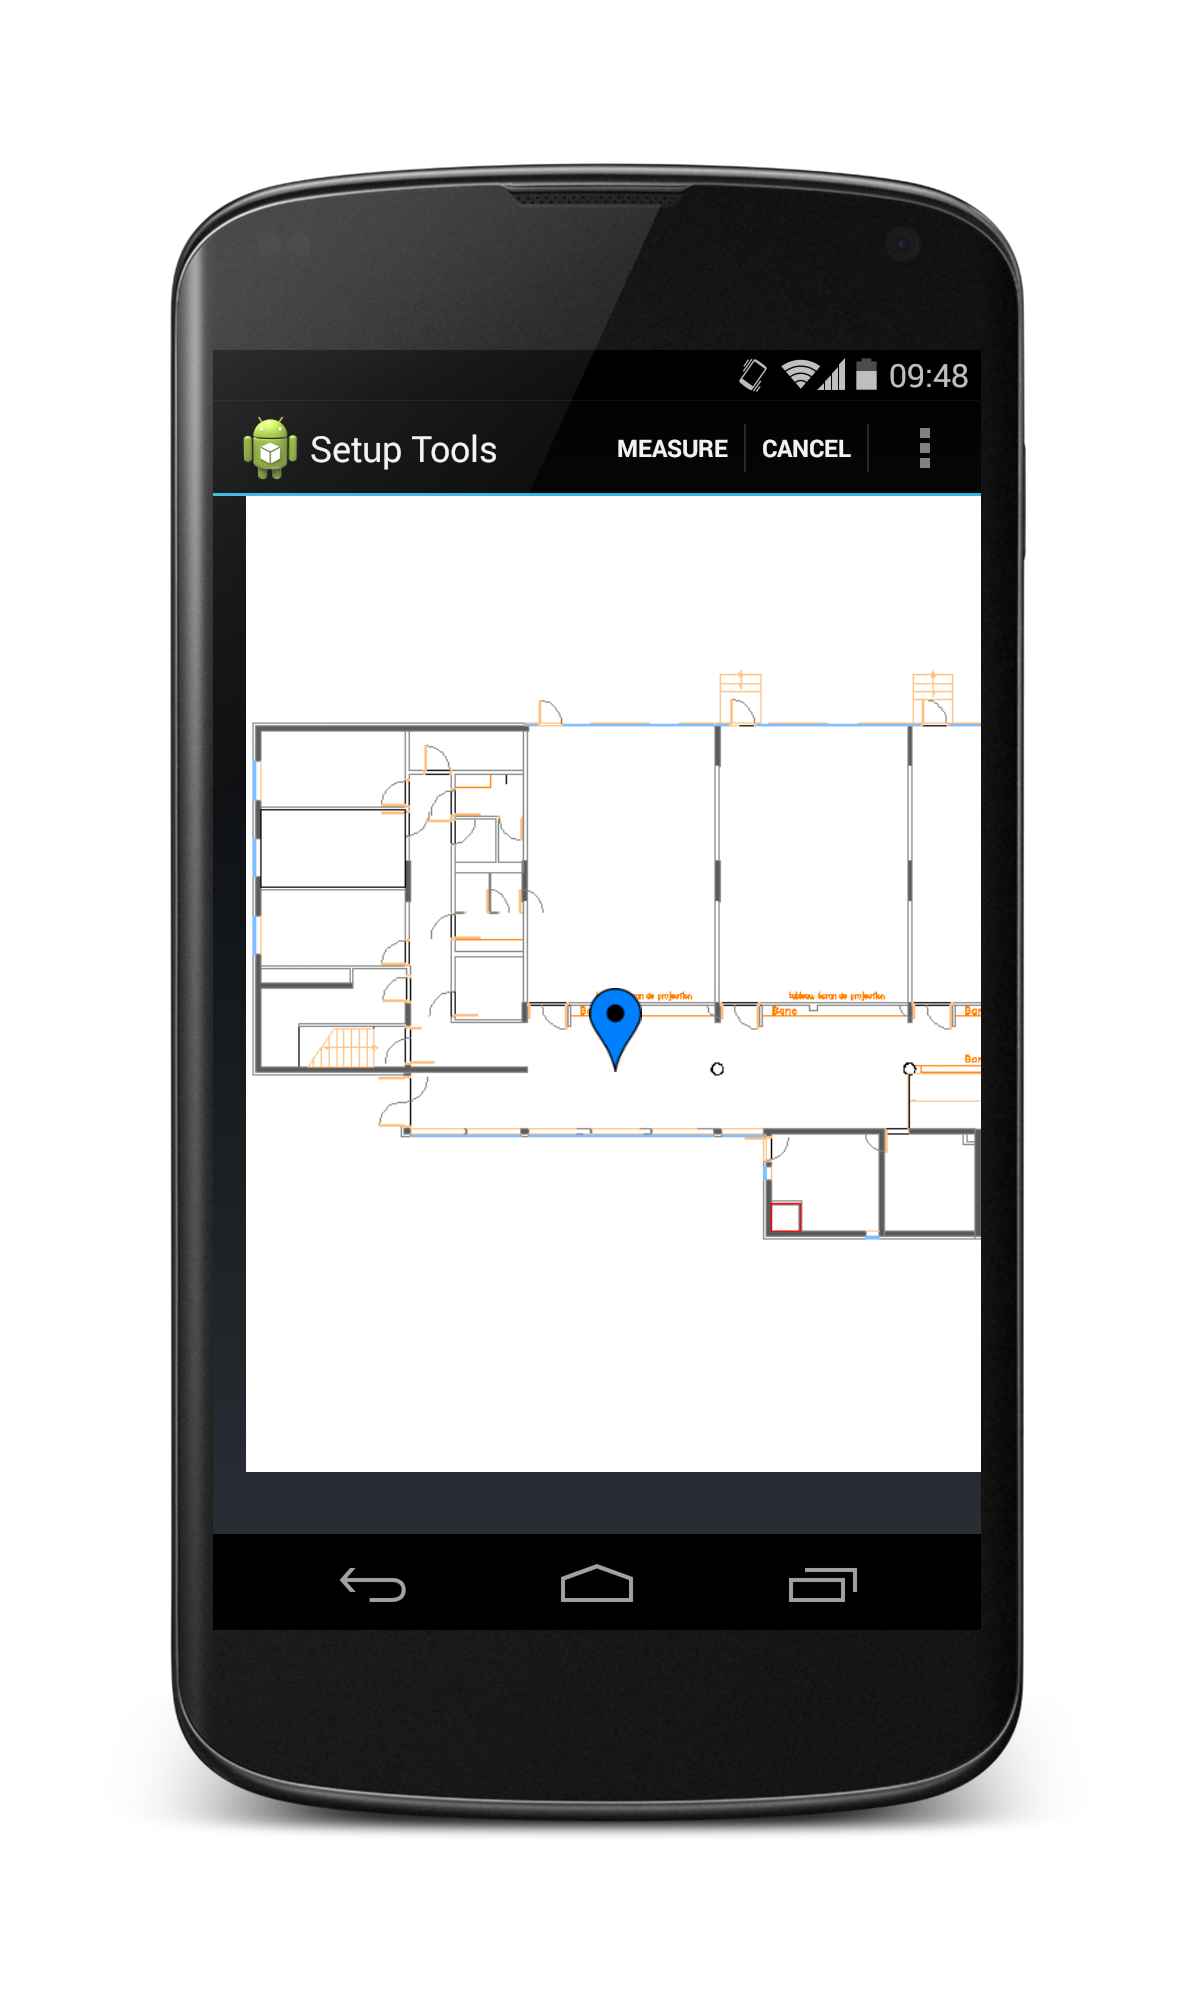
\includegraphics[scale=0.1]{./android/Setup.png}
                \caption{Set calibration point}
                \label{fig:map}
        \end{subfigure}
        \caption{Setup Tools application}\label{fig:setup}
\end{figure}

\begin{itemize}
\item First, when you launch the application there is a list of all map available on the server which is displayed. It contains the id, a description and the size of the map in meters. Then you just have to select the correct one. It is also possible, when you know the id of the map to use the search bar. Indeed you just have to put the correct id and it will display the map just like if you choose it from the list. (See Figure \ref{fig:map_list})
\item Then when the map is displayed you have to click on the "set" button to be able to add a calibration point. (See Figure \ref{fig:map_set})
\item Once you clicked on the "set" button you can set your calibration point and click on "measure" to send all the information to the server. It's also possible to cancel using the "cancel" button which remove your calibration point (on the map). (See Figure \ref{fig:setup})
\end{itemize}

\section{Positioning}
Now we will talk about the positioning application which allow a user to be located in a building according to the calibration points set with the previous application.

\begin{figure}[h!]
  	\centering
    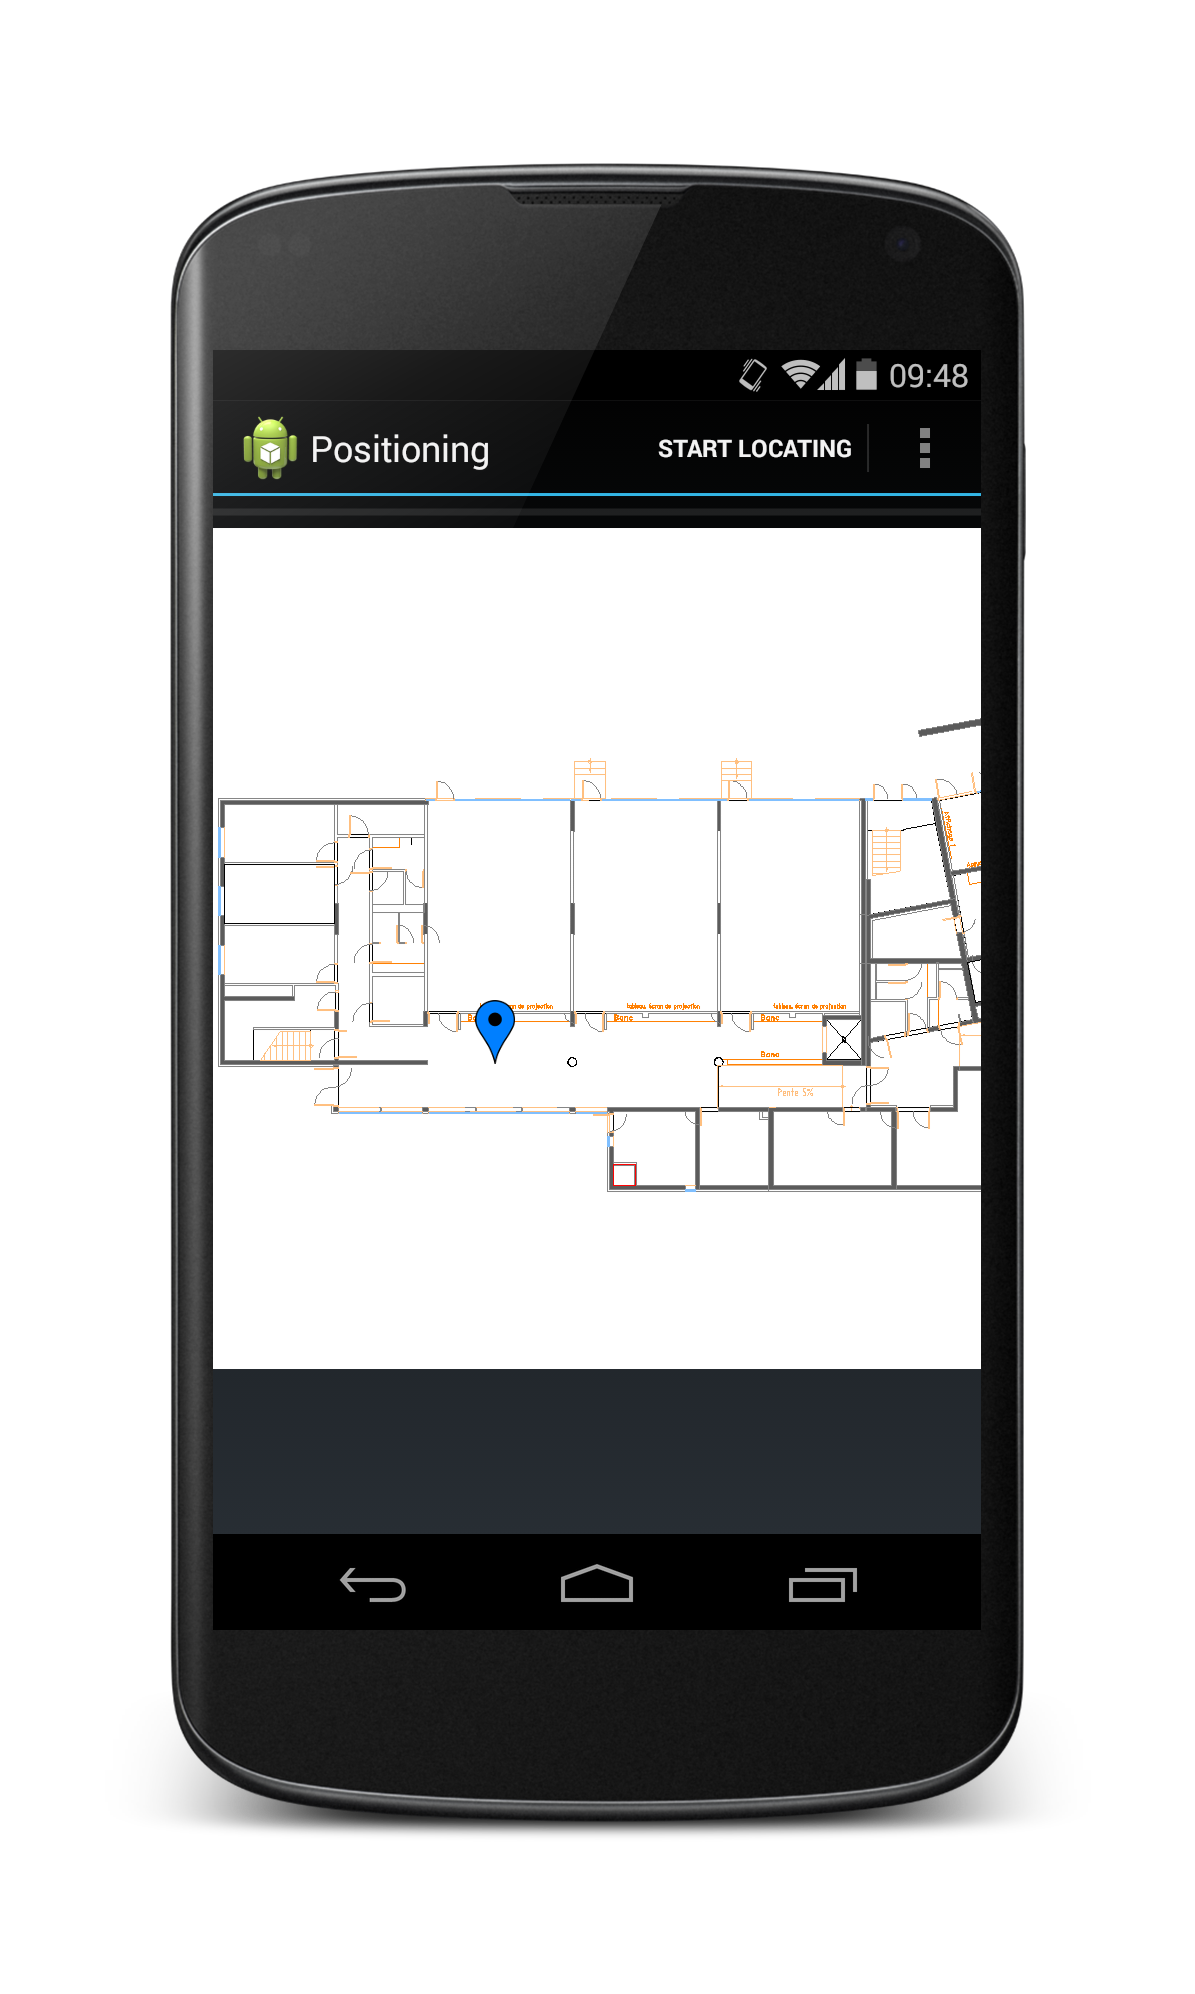
\includegraphics[scale=0.1]{./android/Positioning.png}
  \caption{Positioning application}
\end{figure}

This application is very simple. The user just have to click on "Start locating" and the application sends a positioning request to the server and display the result on the screen (map to display, position).


\section{RSSI values}

For this two applications the access points require a maximum of RSSI values. If the mobile does not communicate, the access points do not retrieve RSSI values which prevents the applications to work correctly. So in both application we ping the server but also launch a wifi scan which allow the access points to retrieve about 50 RSSI values.

